\documentclass[Bachelorarbeit.tex]{subfiles}
\begin{document}
\chapter{Implementierung}
\label{chap:implementierung}

\ideas{Recherche, Auswahl und Implementierung der Standorterfassung von Mitarbeiter\_innen ... Anpassung des bestehenden Systems - eventuell eigener Abschnitt}

 - Datenstrukturen schaffen\\
 - GIS Daten besorgen\\
 - Implementierung der Listenansicht\\
 - Implementierung der Kartenansicht\\
 - No Scroll\\
 - Standort speichern\\
 \\
 - Herausforderungen\\
 / Leaflet.js - Popups, individuelle Marker mit Zahlen


\section{Spezifikation}
\label{chap:implementierung:sec:spezifikation}
\ideas{Beschreibung welche Technologien warum eingesetzt werden sowie die Rahmenbedingungen der Implementierung (Hardware, Software, etc.)}
Im Zuge der vorangegangen Analysen sowie verschiedenen Rahmenbedingung werden folgende Technologien für die Implementierung eingesetzt. 

\subsection*{Programmiersprachen}
Grundsätzlich wird der Prototyp auf Serverseite mit Python in der Version 2.7 realisiert. 
Dabei handelt es sich viel mehr um eine Vorgabe, da der Prototyp innerhalb des bestehenden Systems Pery integriert wird und Pery selbst mithilfe des Webframeworks Django entwickelt wird welches in Python geschrieben ist.
Bei Python handelt es sich um 
\ideas{kurze Info über Python und seine Besonderheiten}

Ergänzend zu Python wird auf der Seite des Clients teilweise Java Script eingesetzt. 

\subsection*{Webframeworks}
Im speziellen spielen die Frameworks Django 

/url conf
/admin
/view

\section{Details zur Implementierung}
\label{chap:implementierung:sec:details}
\ideas{Besondere Aspekte etc. der Implementierung aufzeigen - mit Relevanz zum Kapitel \nameref{chap:entwicklung}}

\subsection{Implementierung Serverseite}
Anhand des Sequenzdiagrammes (siehe Abbildung \ref{fig:Overview}) soll ein  Überblick über den Standardablauf auf der Serverseite vermittelt werden. 
Sobald die Anwender\_innen im  Prototyp auf den Link edit trip klicken wird eine  Anfrage an den Webserver gesendet.
Der Webserver bereitet die erhaltenen Daten auf und leitet sie an die Admin-Seite des Trips (TripAdmin) weiter (siehe Abbildung \ref{fig:Overview} - 1.1 request). 
Die Funktion Planning Trip Action des TripAdmins wird dabei aufgerufen und die entsprechende View (TripBase) geladen (siehe Abbildung \ref{fig:Overview} - 1.1.1.1 - initial TripBase).
Innerhalb der View werden bis zur Rücksendung der Antwort (Response) an den Web Server die drei Funktionen prepare, render\_output und render\_to\_response durchlaufen
Dabei wird in der Funktion prepare (siehe Abbildung \ref{fig:Overview} - 1.1.1.1.1) hauptsächlich die \ac{AJAX}-Funktionalität aktiviert.
Die benötigten Daten werden in der Funktion render\_output (siehe Absatz \nameref{renderOutput}) aus der Datenbank geladen und entsprechend vorbereitet bis sie anschließend an die Funktion render\_to\_response oder über das \ac{AJAX}-Framework (nicht in der Abbildung) an den Webserver weitergeleitet werden.
In der Funktion render\_to\_response (siehe Abbildung \ref{fig:Overview} - 1.1.1.1.3) werden die definierten Templates mit Hilfe der erhaltenen Daten, mithilfe des Django-Frameworks, in das \ac{HTML}-Format übertragen und in einen Response eingebettet.
Abschließend wird der generierte Response an den Webserver weitergegeben der ihn schlussendlich an den Web Browser ausliefert.


\begin{figure}[h]
\centering
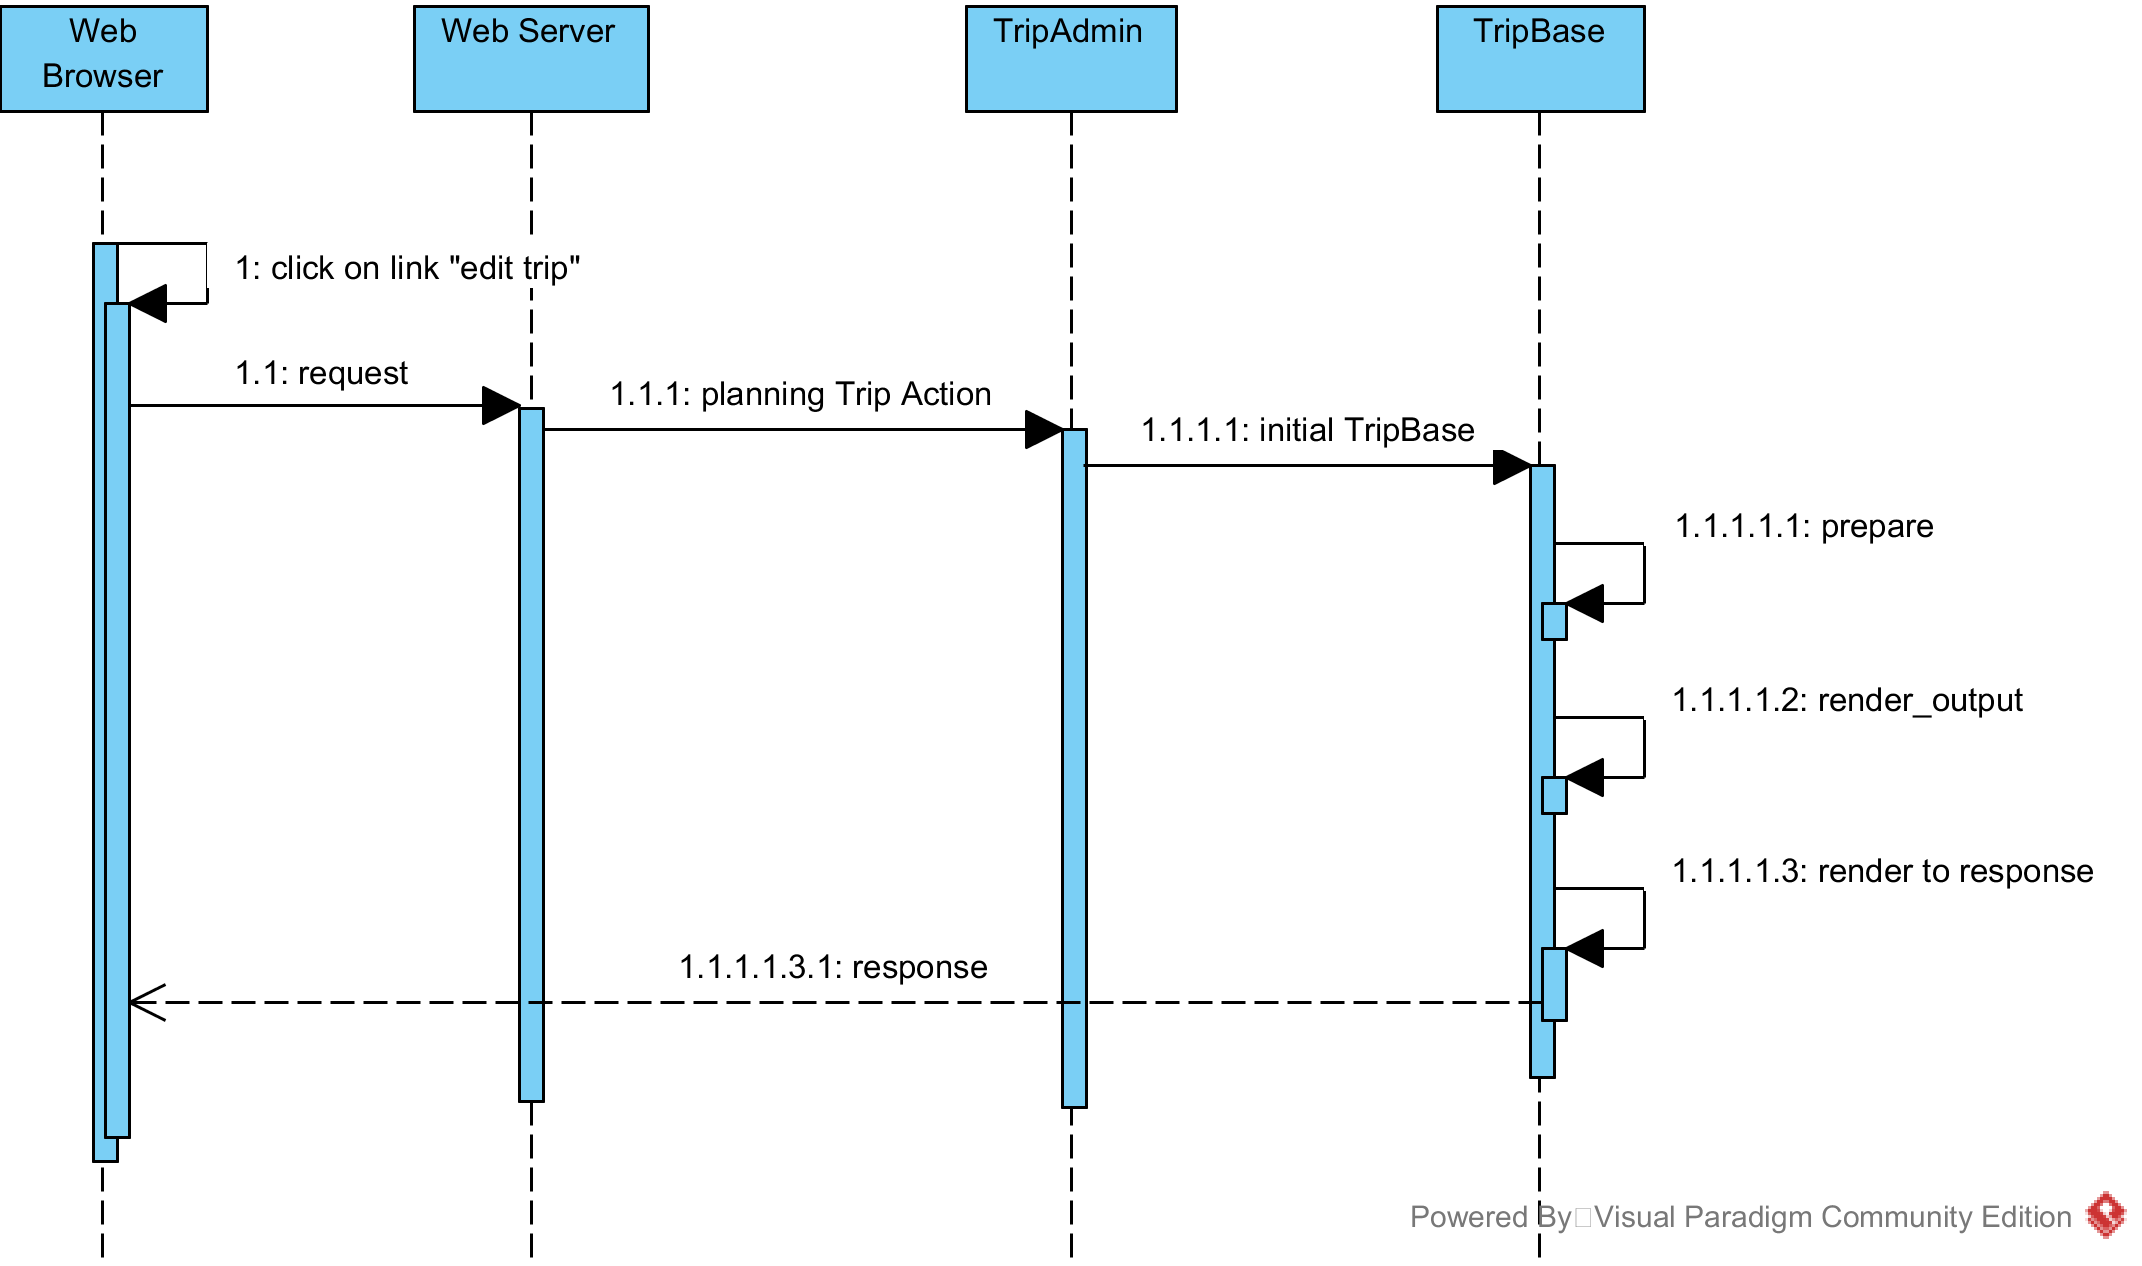
\includegraphics[width=1\linewidth]{img/Implementierung/Overview}
\caption[k]{Sequenzdiagramm: Übersicht des Ablaufs vom Request bist zum Response. Quelle: eigene Ausarbeitung.}
\label{fig:Overview}
\end{figure}

\subsubsection*{Funktion: render\_output}
\label{renderOutput}
Nachdem die Funktion prepare in der TripBase View abgeschlossen ist wird die Funktion render\_output gestartet (siehe Abbildung \ref{fig:Overview} - 1.1.1.1.2).
Beginnend mit dem Auslesen des PresantationMode's aus dem Request, welcher als Parameter übergeben wird, wird definiert ob die Karten oder Listenansicht erstellt werden soll (siehe Abbildung \ref{fig:renderOutput} - 1.).
Sollte das Auslesen nicht möglich sein, weil der Trip beispielsweise das erste Mal aufgerufen wird, so wird die Kartenansicht als Standartwert verwendet.
Sollte es sich bei dem Request um einen \ac{AJAX}-Aufruf handeln so wird dieser, je nach Bedarf abgewickelt und als Response an den Webserver zurück geschickt.
Anschließend werden mittels der Datenbank Abstraktion alle Tripstations\footnote{Tripstations sind Unternehmen welche bereits dem Trip hinzugefügt wurden.} geladen (siehe Abbildung \ref{fig:Overview} - 2. bis 2.3).
An dieser Stelle teilt sich der weitere Ablauf auf, je nach dem welcher PresantationMode gewählt wurde und es sich nicht um einen \ac{AJAX}-Aufruf handelt (siehe Abschnitte \nameref{PERYMapTrip} und \nameref{PERYListTrip}).\\


\paragraph{Rank}
\label{Rank}
Damit der Ablauf in der Kartenansicht besser verständlich wird, muss im Vorfeld die Verwendung und der Aufbau der Rank's geklärt werden.
Im Vorfeld wurde definiert das die Marker der Karte, durch die Verwendung unterschiedlicher Farben, zusätzliche Informationen zu den Unternehmen transportieren sollen, wie Beispielsweise Gesamtumsatz oder letzer Besuch.
Dafür müssen die Daten entsprechend vorbereitet und über Funktionen der Visualisierung zur Verfügung gestellt werden. \\
\\
Um dies zu realisieren wurde die Klasse PeryDataRank geschrieben (siehe Abbildung \ref{fig:ClassDiagrammRank}). 
Innerhalb der View (TripBase), wird für jeden Rank (Gesamtumsatz, letzer Besuch, etc.) ein Objekt der Klasse PeryDataRank erstellt (available\_ranks).
Dabei wird über die Attribute des Objektes (clazz:string und attr:string) gesteuert woher die Daten für diesen Rank kommen sollen. \\

\begin{figure}[H]
\centering
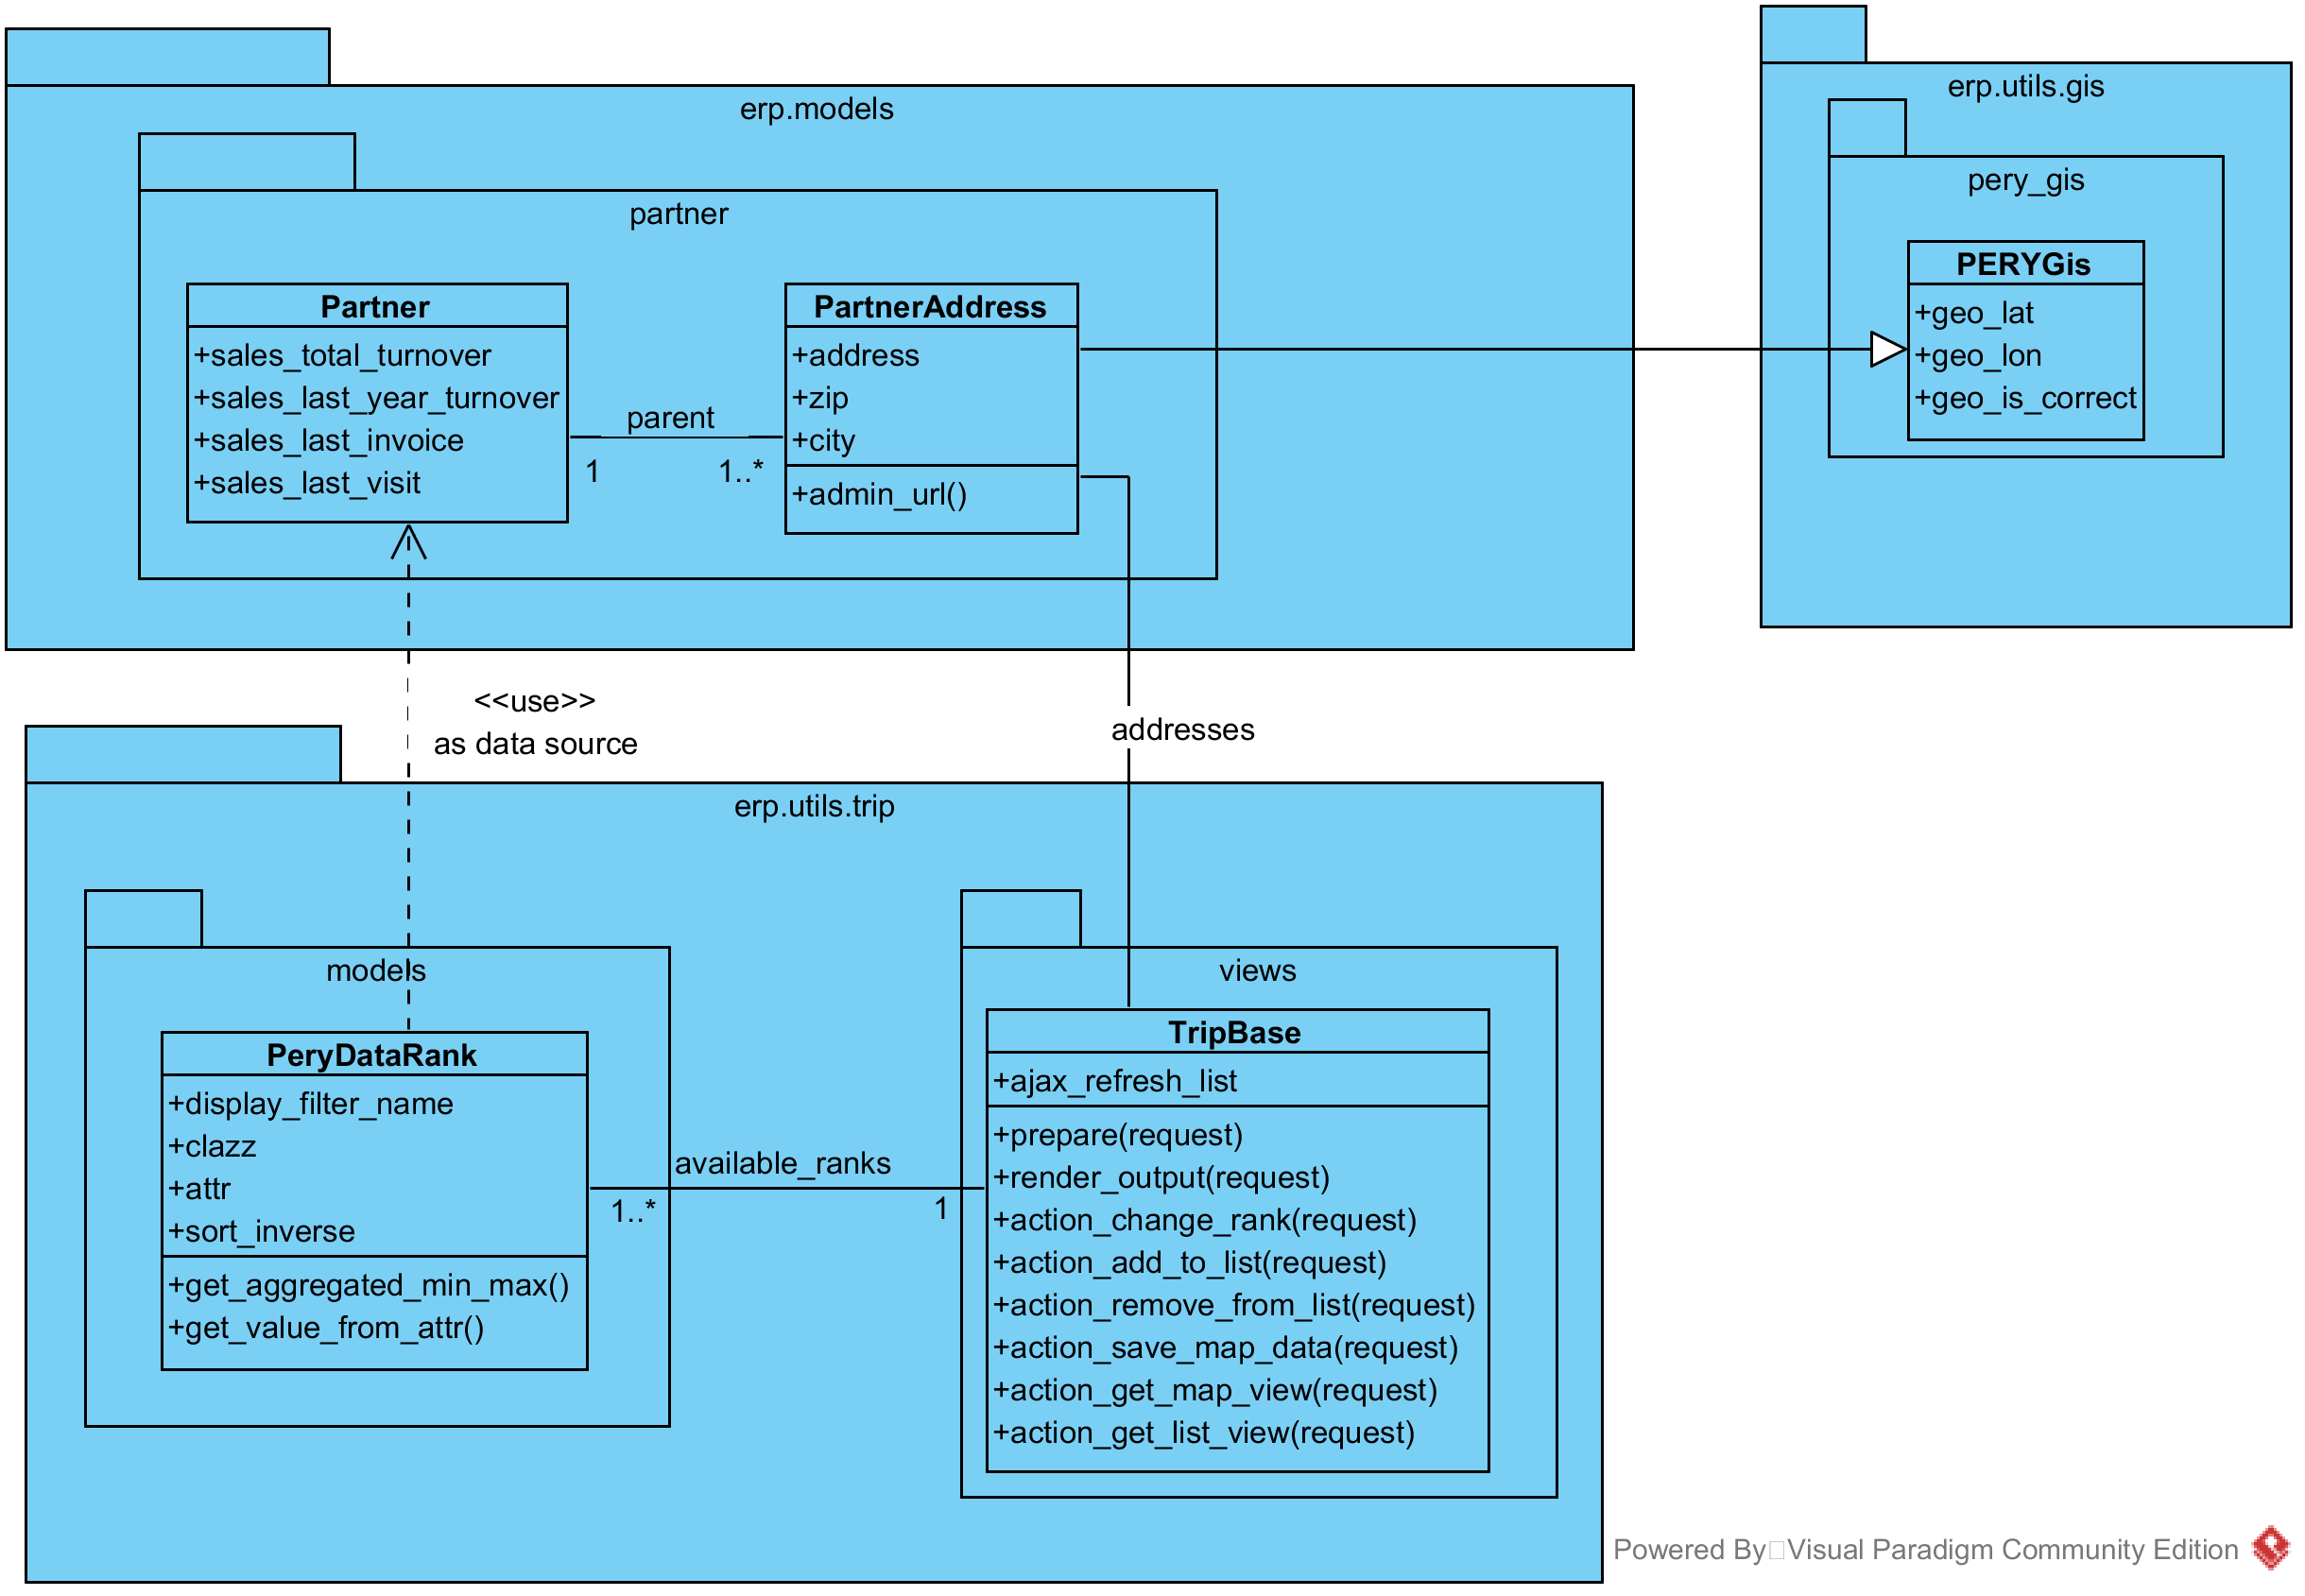
\includegraphics[width=0.9\linewidth]{img/Implementierung/ClassDiagrammRank}
\caption[k]{Klassendiagramm: PeryDataRank. Quelle: eigene Ausarbeitung.}
\label{fig:ClassDiagrammRank}
\end{figure}

Dabei ist anzumerken das die verfügbaren Rank's (available ranks), als Dictionary mit dem Datentyp PeryDataRank, auf Klassenebene der View (TripBase) definiert werden.

\paragraph{PERYMapTrip}
\label{PERYMapTrip}
Im Fall der Kartenansicht wird ein Objekt der Klasse PERYTripMap initialisiert. 
Anschließend werden, mittels der Datenbank Abstraktionen alle Objekte der Klasse PartnerAddress geladen welche über Daten in den Attributen geo\_lat und geo\_lon verfügen (siehe Abbildung \ref{fig:Overview} - 4. bis 4.3). \\
\\
Um die Marker auf der Karte später nach dem ausgewählten Rank (Beispielsweise Gesamtumsatz oder letzer Besuch) entsprechend einzufärben muss der Rank noch korrekt erstellt werden (siehe Abschnitt \nameref{Rank}). 
Dafür wird im ersten Schritt der aktive Rank aus den Request Parametern ausgelesen und verglichen ob er verfügbar ist.
Mittels einer Funktion wird aus dem aktiven PeryDataRank die entsprechenden min. und max. Werte (Bsp. letzter Besuch) aus dem dazugehörigen Partner Objekten
	\footnote{Auf die Partner Objekte wird über den Fremdschlüssel in dem PartnerAddress Objekt zugegriffen (siehe Abbildung \ref{fig:ClassDiagrammRank})}  
berechnet (siehe Abbildung \ref{fig:renderOutput} - 5.).
Anhand der berrechneten min. und max. Werte sowie der gegeben Anzahl an Abstufungen (Range) können nun Ranges eingeteilt und an die Karte (PERYTripMap) weitergegeben werden.
	\footnote{Beisoiel: Der aktive Rank ist Gesamtumsatz. Dabei belaufen sich die min. und max. Werte auf 0 Euro bis 10.000 Euro, die Anzahl der Ranges entspricht 5. Somit fallen die Unternehmen mit einem Gesamtumsatz von 0 Euro bis 2000,00 Euro in Range 1, von 2000,01 Euro bis 4000,00 Euro in Range 2, ..., von 8000,01 Euro bis 10.000,00 Euro in Range 5.} 
Nun wird für alle PartnerAddress, welche zuvor aus der Datenbank gelesen wurden, jeweils die Funktion addPoint des PERYMapTrip  aufgerufen. 
Diese Funktion erzeugt im ersten Schritt einen neuen PeryMapPoint, welcher alle Informationen (Koordinaten, Daten für das Popup, etc.) besitzt die für die Visualisierung auf der Karte notwendig ist.
Im zweiten Schritt wird das neue Objekt klassifiziert.  
Anhand seines Rank-Wertes wird das Objekt in eine der zuvor definierten Ranges eingeteilt (siehe Abbildung \ref{fig:renderOutput} - 7. bis 7.3).

\paragraph{PERYListTrip}
\label{PERYListTrip}
Sollte die Listenansicht ausgewählt sein wird der vorhergehende Abschnitt durch diesen ersetzt.
Dabei wird im ersten Schritt ein Objekt der Klasse PERYListTrip in der View (TripBase) angelegt.
Anschließend werden die PartnerAddresses Objekte aus der Datenbank geladen und der Sammlung im PERYListTrip hinzugefügt (siehe Abbildung \ref{fig:renderOutput} - 9. bis 10.).



\begin{figure}[h]
\centering
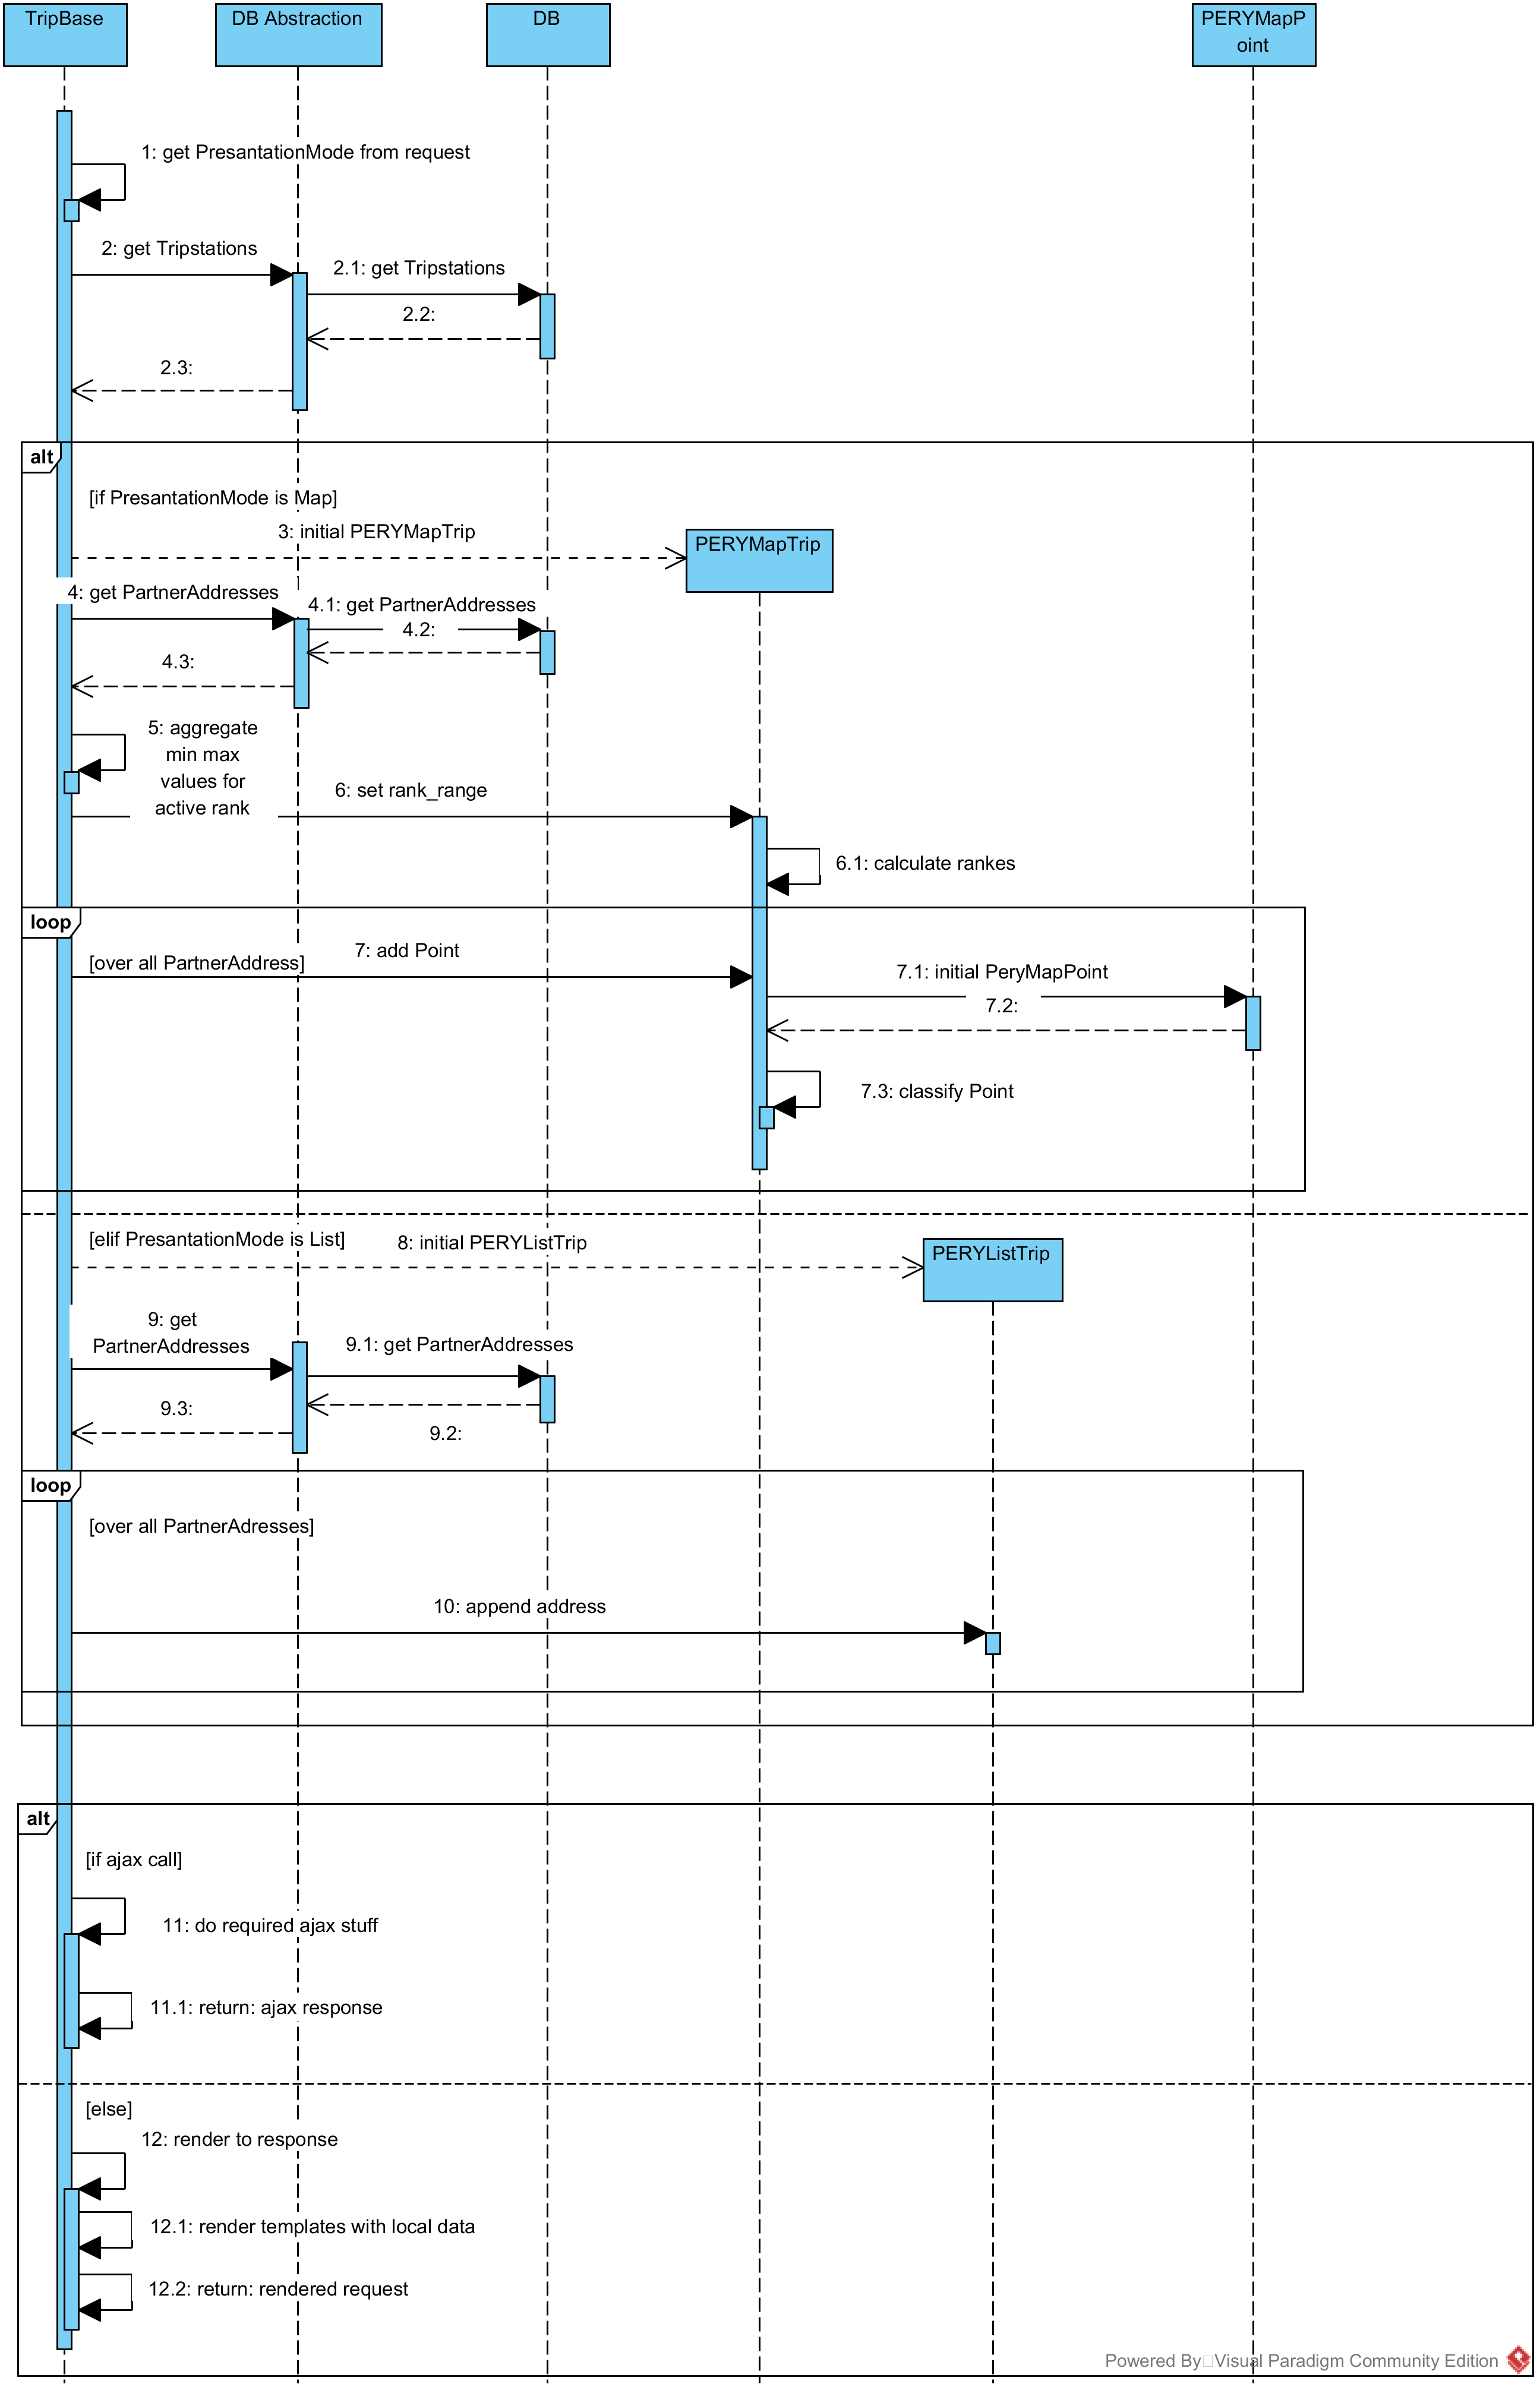
\includegraphics[width=1\linewidth]{img/Implementierung/renderOutput}
\caption[k]{Sequenzdiagramm: Ablauf der Funktion render\_output auf dem Server. Quelle: eigene Ausarbeitung.}
\label{fig:renderOutput}
\end{figure}

\subsection{Implementierung Clientseite}

\subsection{Probleme bei der Implementierung}
/ Probleme
/ SVG -- dyn. Marker
\end{document}